\documentclass{beamer}


\usetheme{light}

\usepackage{adjustbox}


\title{Presentation Title}
\subtitle{Subtitle}
\author{Eric D. Weise}
% \institute[]{}
\date{}
% \subject{}


\begin{document}

	\frame {
        \titlepage
	}

	\frame {
		\frametitle{Outline}
		\tableofcontents
	}

	\section[Section]{Section 1}
	
	\frame {
        \frametitle{Page 1}
        \framesubtitle{Example of Text}

		Contents...
	}

	\section[Section]{Section Two}

	\frame{
		\frametitle{Page 2}
		\framesubtitle{Example of Lists}

		\begin{itemize}
			\item 1
			\item 2
			\item 3
		\end{itemize}
	}

	\subsection[Subsection]{Subsection 2.1}

	\frame{
		\frametitle{Two Column Slide}

		\begin{columns}
		\column{0.5\textwidth}
			This is a text in first column.
			$$E=mc^2$$
			\begin{itemize}
			\item First item
			\item Second item
			\end{itemize}
		\column{0.5\textwidth}
			This text will be in the second column.
			It can also include an image.
		\end{columns}
	}

	\frame{
		\frametitle{An Example Photo}

		\centering
		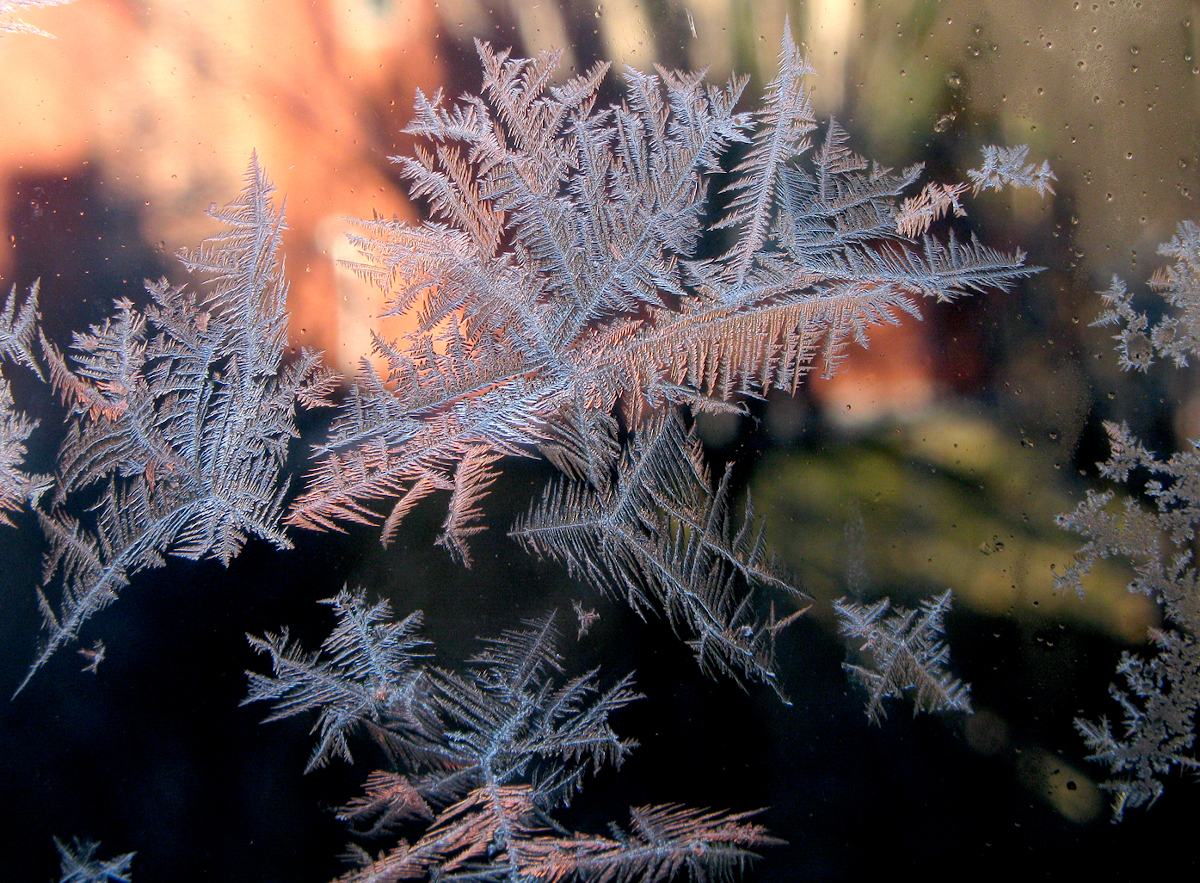
\includegraphics[keepaspectratio=true, scale=0.4]{../assets/images/icecrystals.jpg}
	}

\end{document}
